\textbf{Ejemplo 6}\\
Una industria puede adquirir una maquina a un costo de 6 millones COP, tendrá una vida útil de 5 años y prácticamente no tendrá valor de salvamento, la máquina será depreciada totalmente en 3 años por partes iguales; el estudio de mercados indica que los ingresos del primer año serán aproximadamente de 3 millones COP y aumentarán todos los años un 30\%, por otra parte se estima que el costo de producción del primer año será de 800.000 COP y cada año aumentará en 200.000 COP. Suponiendo una tasa impositiva del 38\%, determinar la viabilidad del proyecto con un horizonte de planeación de 5 años y que la tasa del inversionista es del 40\%.\\


%%%%%%%%%%%%%%%%%%% EJERCICIO 7 %%%%%%

%\newpage %USAR SOLO SI EL SOLUCION QUEDA SOLO Y ES NECESARIO BAJARLO A LA SIGUIENTE PAGINA
\textbf{Solución.}\\
%La tabla ira centrada
\begin{center}
	\renewcommand{\arraystretch}{1.5}% Margenes de las celdas
	%Creacion de la cuadricula de 3 columnas \end{flushleft}
	\begin{longtable}[H]{|C{0.3\linewidth}|C{0.3\linewidth}|C{0.3\linewidth}|}
		%Creamos una linea horizontal
		\hline
        %%%%% INICIO FLUJO DE CAJA
		\rowcolor[HTML]{FFB183}
		\multicolumn{3}{|c|}{\cellcolor[HTML]{FFB183}\textbf{1. Asignación periodo focal}}   \\ \hline
		\multicolumn{3}{|c|} {$pf = 0 pav$} \\ \hline
		%%%%%%%%%% FIN TITULO
		%%%%%%%%%% INICIO TITULO
		%Lo que se hace aqui es mezclar las 3 columnas en una sola
		\multicolumn{3}{|c|}{\cellcolor[HTML]{FFB183}\textbf{2. Declaración de variables}}   \\ \hline
		%%%%%%%%%% FIN TITULO
		%%%%%%%%%% INICIO DE MATEMATICAS
		%Cada & hace referencia al paso de la siguiente columna
		$S=  6.000.000$ COP & $VS= 0$ COP & $n= 5 pav$\\
		$IngresoS =3.000.000$ COP & $i_{i}= 30\% pav$ & $C= 800.000 $ COP\\
		$Aumento  C= 200.000 $ COP & $i_{impositiva}= 38\% pav$ & $i_{inversionista}= 40\% pav$\\
		%%%%%%%%%% FIN DE MATEMATICAS
		%%%%% FIN DECLARACION DE VARIABLES

  		%%%%% INICIO DECLARACION FORMULAS
  
		%%%%%%%%%%% INICIO TITULO
		\rowcolor[HTML]{FFB183}
		\multicolumn{3}{|c|}{\cellcolor[HTML]{FFB183}\textbf{3. Diagrama de flujo de caja}} \\ \hline
		%Mezclamos 3 columnas y ponermos el dibujo
		%%%%%%%%%%%%% INSERCION DE LA IMAGEN
		%Deberan descargar las imagenes respectivas del drive y pegarlas en la carpeta
		%n_capitulo/img/ejemplos/1/capitulo1ejemplo1.pdf  (el /1/ es el numero del ejemplo) 
		\multicolumn{3}{|c|}{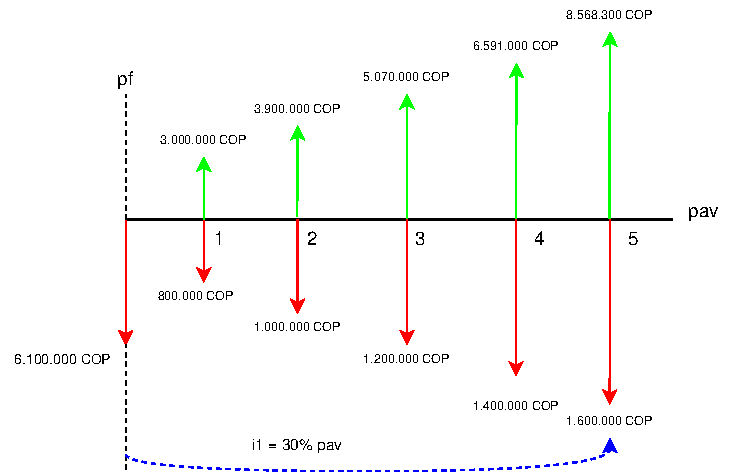
\includegraphics[trim=-5 -5 -5 -5 , scale=1, width=300px, height=250px]{9_Capitulo/ejemplos/7/Capitulo9Ejercicio7.pdf}}  \\ \hline
		%%%%%%%%%%%%% FIN INSERCION DE IMAGEN
		%%%%%FIN FLUJO DE CAJA



		%%%%% INICIO DECLARACION FORMULAS
		%%%%%%%%%%% INICIO TITULO
		\rowcolor[HTML]{FFB183}
		\multicolumn{3}{|c|}{\cellcolor[HTML]{FFB183}\textbf{4. Declaración de fórmulas}}    \\ \hline
		%%%%%%%%%%% FIN TITULO
		%%%%%%%%%%% INICIO MATEMATICAS
		\multicolumn{3}{|c|}{$Flujo\_neto\_de\_caja= Ingresos - Cosos - Impuestos$}\\
		\multicolumn{3}{|c|}{$Impuestos=Tasa\_impositiva*Base$}\\
		\multicolumn{3}{|c|}{$Base = Ingreso - Costos - Depreciacion$} \\
		\multicolumn{3}{|c|}{$\sum F_{n}(1+i)^{-n} $\hspace{0.3cm} \textit{Valor presente neto}} \\ \hline
		%%%%%%%%%% FIN MATEMATICAS
		%%%%%% INICIO DESARROLLO MATEMATICO
		\rowcolor[HTML]{FFB183}
		%%%%%%%%%%INICIO TITULO
		\multicolumn{3}{|c|}{\cellcolor[HTML]{FFB183}\textbf{5. Desarrollo matemático}}       \\ \hline
		%%%%%%%%%% FIN TITULO
		%%%%%%%%%% INICIO MATEMATICAS
		
        		\multicolumn{3}{|c|}{
		\resizebox{\textwidth}{!}{%
        			\begin{tabular}{ |c | c |c |c | c |c | c |} 
                    		\hline
                    		PERIODO & INGRESO     & COSTO       & DEPRECIACIÓN & BASE        & IMPUESTO    & FNC         \\
                    		\hline
                    		0       & 6.000.000 COP & 0 COP        & 0 COP         & 0 COP        & 0 COP        & 6.000.000 COP \\
                    		\hline
                    		1       & 3.000000 COP  & 800.000 COP   & 2.000000 COP   & 200.000 COP   & 7.6000 COP    & 2-124.000 COP \\
                    		\hline
                    		2       & 3.900.000 COP & 1.000.000 COP & 2.000.000 COP  & 900.000 COP   & 342.000 COP   & 2.558.000 COP \\
                    		\hline
                    		3       & 5.070.000 COP & 1.200.000 COP & 2.000.000 COP  & 1.870.000 COP & 710.600 COP   & 3.159.400 COP \\
                    		\hline
                    		4       & 6.591.000 COP & 1.400.000 COP & --           & 5.191.000 COP & 1.972.580 COP & 3.218.420 COP \\
                    		\hline
                    		5       & 8.568.300 COP & 1.600.000 COP & --           & 6.968.300 COP & 2.647.954 COP & 4.320.346 COP \\
                    		\hline
            		\end{tabular}}
		}\\ 
	
		\multicolumn{3}{|c|}{$VPN = -6.000.000+2.124.000(1+0.4)^{-1}+2..558.000(1+0.4)^{-2}$}\\
		\multicolumn{3}{|c|}{$+3.159.400(1+0.4)^{-3}+3.218.420(1+0.4)^{-4}+4.320.346(1+0.4)^{-5}$} \\
		\multicolumn{3}{|c|}{$VPN=-385.288 $ COP}\\ \hline

		%%%%%%%%%% FIN MATEMATICAS
		%%%%%% FIN DESARROLLO MATEMATICO
		%%%%%% INICIO RESPUESTA
		\rowcolor[HTML]{FFB183}
		%%%%%%%%%%INICIO TITULO
		\multicolumn{3}{|c|}{\cellcolor[HTML]{FFB183}\textbf{6. Respuesta}}   \\ \hline
		%%%%%%%%%% FIN TITULO
		%%%%%%%%%% INICIO RESPUESTA MATEMATICA
		\multicolumn{3}{|c|}{El proyecto no resulta ser viable, ya que en la ventana de tiempo dado resultaría en pérdidas.}  \\ \hline
		%%%%%%%%%% FIN MATEMATICAS
		%%%%%% FIN RESPUESTA
	\end{longtable}
	%Se crean dos lineas en blanco para que no quede el siguiente texto tan pegado
	%\newline \newline %USARLO SI CREES QUE ES NECESARIO
\end{center}
%%%%%%%%%%%%%%%%%%%%%%%%%%FIN EJERCICIO 1 %%%%%%%%%%%%%%%%%%%%%%%%%%%
